\section{Power management}

\subsection{Supply filter}

The purpose of the supply filter is to filter out noise from the power supply and buffer voltage peaks.
A simple embodiment of a supply filter is that of an RC low-pass filter as illustrated in \Cref{fig:filter_lowpass}.
\begin{figure}[H]
	\centering
	\begin{circuitikz}
		\draw (0, 0) node[ocirc, label=$V_\text{in}$]{} to[resistor, label=$R$] ++(4, 0) node(node)[circ]{};
		\draw (node) -- ++(2, 0) node[ocirc, label=$V_\text{out}$]{};
		\draw (node) to[capacitor, label=$C$] ++(0, -2) node[ground]{};
	\end{circuitikz}
	\caption{Passive low-pass filter using an RC circuit.}\label{fig:filter_lowpass}
\end{figure}
In \Cref{fig:filter_lowpass} the input voltage is connected through a resistor $R$ with the output voltage.
After the resistor $R$, a capacitor $C$ is connected with ground.
The transfer function of the RC low-pass filter can be obtained from the voltage divider with complex impedances,
\begin{equation}
	\frac{V_\text{out}}{V_\text{in}}
	=\frac{Z_C}{Z_R+Z_C}
	=\frac{1}{1+j\omega RC}.
	\label{eq:transfer_filter_rc}
\end{equation}
The absolute value of the transfer function,
\begin{equation}
	\abs{\frac{V_\text{out}}{V_\text{in}}}
	=\frac{1}{\sqrt{1+\left(f/f_{RC}\right)^2}},
\end{equation}
has a pole at frequency,
\begin{equation}
	f_{RC}=\frac{1}{2\pi RC}.
\end{equation}
% TODO: explain how to select R and C values for low-pass
The frequency response of an RC low-pass with pole frequency $f_{RC}=\SI{100}{\hertz}$ is visualized in \Cref{fig:bode_filter_rc}.
\begin{figure}[H]
	\centering
	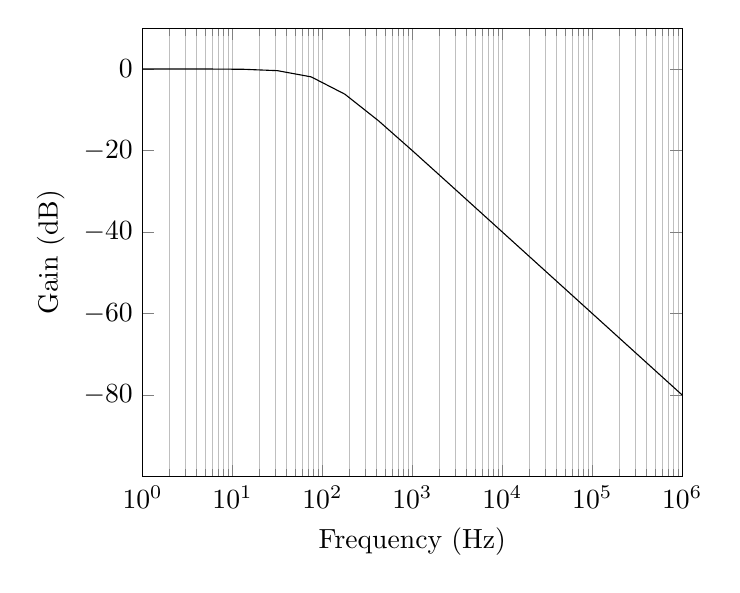
\begin{tikzpicture}
		\begin{semilogxaxis}[xmin=1, xmax=1e6, xlabel=Frequency (Hz), ymin=-100, ymax=10, ylabel=Gain (dB), ytick={0, -20, -40, -60, -80}, grid=minor]
			\addplot[domain=1:1e9]{-10*log10(1+(x/100)^2)};
		\end{semilogxaxis}
	\end{tikzpicture}
	\caption{Bode plot of the frequency response of an RC low-pass at \SI{100}{\hertz}.}\label{fig:bode_filter_rc}
\end{figure}
We can see how the frequency response suppresses frequency above \SI{100}{\hertz}.
However, efficient frequency suppression starts at \SI{-80}{\decibel} which the given RC low-pass of \Cref{fig:bode_filter_rc} only satisfies for much higher frequencies than the pole frequency.

% TODO: give example of two pole filter and how to choose parameters
One approach to improve the frequency response of a filter is to introduce additional frequency poles.
In the limit of infinite many frequency poles, one is able to approach an ideal brick-wall filter.
The frequency response of an ideal brick-wall filter resembles a step function.
In practice, one finds good enough results for two pole filters.

% TODO: give example of capacitance multiplier and how to choose parameters
In addition to a multi-pole filter, a capacitance multiplier can be used to increase the effective capacitance of a filter.
The capacitance multiplier is described in Ref.~\cite[p.~536]{Hobbs11} and Ref.~\cite[p.~578]{Horowitz15}.

\subsection{Voltage regulator}

We use two voltage regulator to maintain a constant voltage of \SI{\pm12}{\volt} which is used to supply the operational amplifiers.

In general, one needs to decide between linear and switching voltage regulators.
Linear voltage regulators are less efficient than their switching counterparts but have better noise characteristics.
As efficiency is not a concern in our application, the better noise characteristics are a strong argument for the linear voltage regulators.
Linear voltage regulators require an input voltage greater than the output voltage.
The difference between input and output voltage is called the drop-out voltage.
The drop-out voltage is about \SIrange{2}{3}{\volt}

Linear voltage regulators are available with fixed and adjustable output voltage.
As we might need an additional voltage drop between the input voltage and the voltage regulator input, e.g. for input power filters, an adjustable voltage regulator would allow for more flexibility.
Moreover, we found the range of negative voltage regulators to be rather limited.

% TODO: working principle (how does R1, R2 on the adjustable terminal change the output voltage?)
\begin{figure}[H]
	\centering
	\begin{circuitikz}
		\draw (0, 0) node[vcc, rotate=90, label={[label distance=6]:\SI[retain-explicit-plus]{+15}{\volt}}]{} -- ++(1, 0) node(node1a)[circ]{} -- ++(4, 0) node(node1b)[circ]{} -- ++(0, 2) to[diode, l_=D1] ++(-4, 0) -- ++(0, -2);
		\draw (node1b) to[resistor, l_=R1, a^=\SI{120}{\ohm}] ++(0, -2) node(node2a)[circ]{} -- ++(-2, 0) -- ++(0, 2);
		\draw (node2a) -- ++(3, 0) node(node2b)[circ]{} to[diode, l=D3] ++(0, 2) node(node1c)[circ]{} -- ++(-3 ,0);
		\draw (node1c) -- ++(2, 0) node(node1d)[circ]{} to[ecapacitor, l_=C5, a^=\SI{1}{\micro\farad}] ++(0, -4) node(node3d)[circ]{} -- ++(-2, 0) node(node3c)[circ]{} -- ++(-3, 0) node(node3b)[circ]{} to[resistor, l^=R2, a_=\SI{980}{\ohm}] ++(0, 2);
		\draw (node2b) to[ecapacitor, l_=C3, a^=\SI{10}{\micro\farad}] (node3c);
		\draw (node1d) -- ++(1, 0) node[vcc, rotate=270, label={[label distance=6]:\SI[retain-explicit-plus]{+12}{\volt}}]{};
		\begin{scope}[xshift=3cm]
			\node[draw, rectangle, fill=white, minimum width=2cm, minimum height=1.2cm, label=U1]{};
			\node at (0, 0) {LM317};
		\end{scope}
		\draw (node3d) -- ++(1, 0) node[ground, rotate=90]{};
		\draw (node3b) -- ++(-5, 0) node[ground, rotate=270]{};
		\draw (node1a) to[ecapacitor, l_=C1, a^=\SI{100}{\nano\farad}] ++(0, -4) node(node3a)[circ]{};
		\draw (node3a) to[ecapacitor, l_=C2, a^=\SI{100}{\nano\farad}] ++(0, -4) node(node5a)[circ]{};
		\draw (node5a) -- ++(-1, 0) node[vee, rotate=270, label={[label distance=6]:\SI{-15}{\volt}}]{};
		\draw (node3b) to[resistor, l_=R3, a^=\SI{980}{\ohm}] ++(0, -2) node(node4b)[circ]{} to[resistor, l_=R4, a^=\SI{120}{\ohm}] ++(0, -2) node(node5b)[circ]{} -- (node5a);
		\draw (node3c) to[ecapacitor, l_=C4, a^=\SI{10}{\micro\farad}] ++(0, -2) node(node4c)[circ]{} to[diode, l_=D4] ++(0, -2) node(node5c)[circ]{} -- (node5b);
		\draw (node3d) to[ecapacitor, l_=C6, a^=\SI{1}{\micro\farad}] ++(0, -4) node(node5d)[circ]{} -- (node5c);
		\draw (node5d) -- ++(1, 0) node[vee, rotate=90, label={[label distance=6]:\SI{-12}{\volt}}]{};
		\draw (node5a) ++(2, 0) -- ++(0, 2) -- (node4b) -- (node4c);
		\begin{scope}[xshift=3cm, yshift=-8cm]
			\node[draw, rectangle, fill=white, minimum width=2cm, minimum height=1.2cm, label=below:U2]{};
			\node at (0, 0) {LM337};
		\end{scope}
		\draw (node5b) -- ++(0, -2) to[diode, l^=D2] ++(-4, 0) -- ++(0, 2);
	\end{circuitikz}
	\caption{Dual supply voltage regulator.}\label{fig:voltage_regulator_dual}
\end{figure}
\Cref{fig:voltage_regulator_dual} illustrates the schematic of the final dual voltage regulator supply circuit.
The input voltage is buffered by capacitors C1 and C2.
U1 and U2 denote the fixed positive and negative voltage regulators.
Resistors R1 and R2 configure the output voltage of U1 to about \SI[retain-explicit-plus]{+11.5}{\volt}.
Resistors R3 and R4 configure the output voltage of U2 to about \SI[retain-explicit-plus]{-11.5}{\volt}.
Capacitors C3, C4, C5 and C6 buffer the output voltage.
When the supply power is switched off and C3 or C5 discharges,
diodes D3 and D1 redirect the current back to the supply lines around the voltage regulators.

\subsection{Voltage reference}

A voltage reference is a high-precision linear (fixed) voltage regulator.
We use it as a voltage source for the sensible reverse bias voltage of the photodiode.
\begin{figure}[H]
	\centering
	\begin{circuitikz}
		\draw (0, 0) node[vcc, rotate=90, label={[label distance=6]:\SI{15}{\volt}}]{} -- ++(1, 0) node(node1a)[circ]{} to[capacitor, l_=C1, a^=\SI{1}{\micro\farad}] ++(0, -4) node(node2a)[circ]{} -- ++(-1, 0) node[ground, rotate=270]{};
		\draw (node1a) -- ++(2, 0) node(node1b)[circ]{} -- ++(0, -4) node(node2b)[circ]{} -- (node2a);
		\draw (node1b) -- ++(2, 0) node(node1c)[circ]{} to[capacitor, l_=C2, a^=\SI{1}{\micro\farad}] ++(0, -4) node(node2c)[circ]{} -- (node2a);
		\draw (node1c) -- ++(2, 0) node(node1d)[circ]{} to[resistor, l_=R1, a^=\SI{100}{\ohm}] ++(0, -2) to[capacitor, l_=C3, a^=\SI{10}{\nano\farad}] ++(0, -2) node(node2d)[circ]{} -- (node2c);
		\draw (node1d) -- ++(2, 0) node(node1e)[circ]{} to[ecapacitor, l_=C4, a^=\SI{22}{\micro\farad}] ++(0, -4) node(node2e)[circ]{} -- (node2c);
		\draw (node1e) -- ++(1, 0) node[vcc, rotate=270, label={[label distance=6]:\SI{10}{\volt}}]{};
		\draw (node2e) -- ++(1, 0) node[ground, rotate=90]{};
		% TODO: use dipchip node and name IC ports
		\begin{scope}[xshift=4cm]
			\node[draw, rectangle, fill=white, minimum width=3cm, minimum height=1.4cm, label=above:U1]{};
			\node at (0, 0) {REF5010};
		\end{scope}
	\end{circuitikz}
	\caption{High-precision voltage reference.}\label{fig:voltage_reference}
\end{figure}
\Cref{fig:voltage_reference} depicts the schematic of the voltage reference circuit.
Capacitor C1 buffers the \SI{15}{\volt} supply voltage.
According to the datasheet the trim terminal should be connected through a capacitor, C2, to ground.
Resistor R1 and capacitor C3 form a low-pass to suppress frequency components in the kHz range.
Finally, capacitor C4 buffers the output voltage.